\chapter{Results}
	
\section{Collective dataset characterization}

In order to apply CCC methods, the publicly available \cite{Hartmann-2021} human colorectal cancer proteomics dataset (acquired via MIBI-TOF) was chosen and analytically explored. The image size of 400 $\mu m^2$ spanned over 1024 pixels\textsuperscript{2} and 36 (phosphorilated) proteins were measured (Supplementary fig. \ref{fig:sup1}, \ref{fig:sup2}). The segmentation masks and annotation into 8 distinct cell-types were provided by the authors. Investigation of the cell-type frequencies showed high variability not only across samples and donors, but also between conditions (Fig. \ref{fig:freq}).
\\[\baselineskip]

\begin{figure}[h!]
    \centering
    \includegraphics[width=16cm]{fig_cell-type_frequency_distributions}
    \caption{\textbf{Cell-type frequency distributions.} (A) Proportion of cell-types across all samples, donors and conditions. (B) Cell-type counts grouped by condition and tumour-immune border presence as defined by \cite{Hartmann-2021}. (C) Proportion of cell-types within a sample for all samples}
    \label{fig:freq}
\end{figure}


Next, the collective dataset (pooled single-cell data across all samples, conditions and donors) was analyzed for general variance, clustering or expression patterns. Mean feature expression was calculated for each feature yielding unique expression patterns for each of the annotated cell-types (Fig. \ref{fig:exploration}A).

Next, variation sources were examined via PCA. The first two principal components of PCA on the pooled single-cell data showed no distinct separation of cells by sample, condition or donor whereas cells of the same cell-type did cluster (Fig. \ref{fig:exploration}B). This indicates low batch effects from these sources and high variance due to cell-types. However, endothelial, myeloid CD68, myeloid CD11c and fibroblast cell-types did not separate as clearly as CD4\textsuperscript{+}, CD8\textsuperscript{+} T cells, endothelial and 'other immune cells'. Since the cell-type accounted for most of the variation, the original pooled feature space of the single-cell data was used for further collective dataset analysis like NCEM. Additionally, performing UMAP on the neighbourhood graph, based on the first 10 principal components of the PCA, showed clustering of the cite{Hartmann-2021} annotated cell-types, where again CD4\textsuperscript{+}, CD8\textsuperscript{+} T cells, endothelial and 'other immune cells' clustered more clearly than endothelial, myeloid CD68, myeloid CD11c cells and fibroblasts.

\begin{figure}[p]
    \centering
    \includegraphics[width=16cm]{fig_global_expression_pca_umap}
    \caption{\textbf{Data exploration of the Hartmann-2021 dataset on pooled single-cell data across samples, donors and conditions.} (A) Feature expression mean was calculated by cell-type and lineage marker across all samples, donors and conditions. (B) Juxtaposed 2-dimensional representation of PCA and UMAP dimensionality reduction coloured by cell-type, donor, sample and condition. The neighbourhood graph and UMAP  were calculated using the first 10 principal components}
    \label{fig:exploration}
\end{figure}


The specific expression profiles of major immune cell lineage markers from the original paper were recovered via the mean expression per cell-type (Fig. \ref{fig:lineage-recovery}A,C). On the UMAP space (Fig. \ref{fig:lineage-recovery}B), it was expected that the expression of the lineage markers would enrich or deplete according to their cell-type. This was observed with the exception of markers CD11c, CD68 and CD31, corresponding to cell-types whose clustering was less clear in the UMAP space. Furthermore a set of 12 highly variable features were obtained that were not part of the lineage-marker set (Supplementary table \ref{tab:sup-hvargs}).

\begin{figure}[h!]
    \centering
    \includegraphics[width=16cm]{fig_lineage_profile_recovery}
    \caption{\textbf{Lineage specific expression profiles of provided cell-type annotation by Hartmann-2021.} (A) The expression mean of major immune lineage specific markers was calculated by cell-type and lineage marker across all samples, donors and conditions. (B) The neighbourhood graph and consecutive UMAP embedding was performed using the first 10 principal components and then coloured by cell-type and (C) by the major immune lineage markers.}
    \label{fig:lineage-recovery}
\end{figure}

\pagebreak



\section{Exploration and characterization of colorectal carinoma and healthy samples}

Next, two arbitrary samples were chosen for an exemplary analysis on an image-level basis.  "Point23" was chosen from the colorectal carcinoma samples with a tumour-immune border (defined as per Hartmann-2021). "Point49" was chosen from the healthy colon samples.

PCA and UMAP were performed on the cancer sample to examine how much cell-type accounts for variation. The first two principal components only accounted for epithelial cell-type separation. UMAP clustered CD4\textsuperscript{+}, CD8\textsuperscript{+} and 'immune other' cells in addition to epithelial cells (Fig. \ref{fig:explor-cancer}A). Plotting the expression of major immune lineage markers under the cell segmentation area revealed the expected spatial distribution and enrichment linked to their cell-type (Fig \ref{fig:explor-cancer}B). In addition, highly variable genes of the sample which differed from the lineage markers were calculated (Supplementary table 1) and the expression under the segmentation mask of CD98, Ki67 and NaKATPase are plotted (Fig \ref{fig:explor-cancer}C). CD98 was expressed towards the cancerous epithelial cells with depletion in the epithelial cells. Ki67 was sparsely expressed in apparently arbitrary cell-types. NaKATPase was found to be enriched towards the cancerous epithelial cells.

\begin{figure}[p]
    \centering
    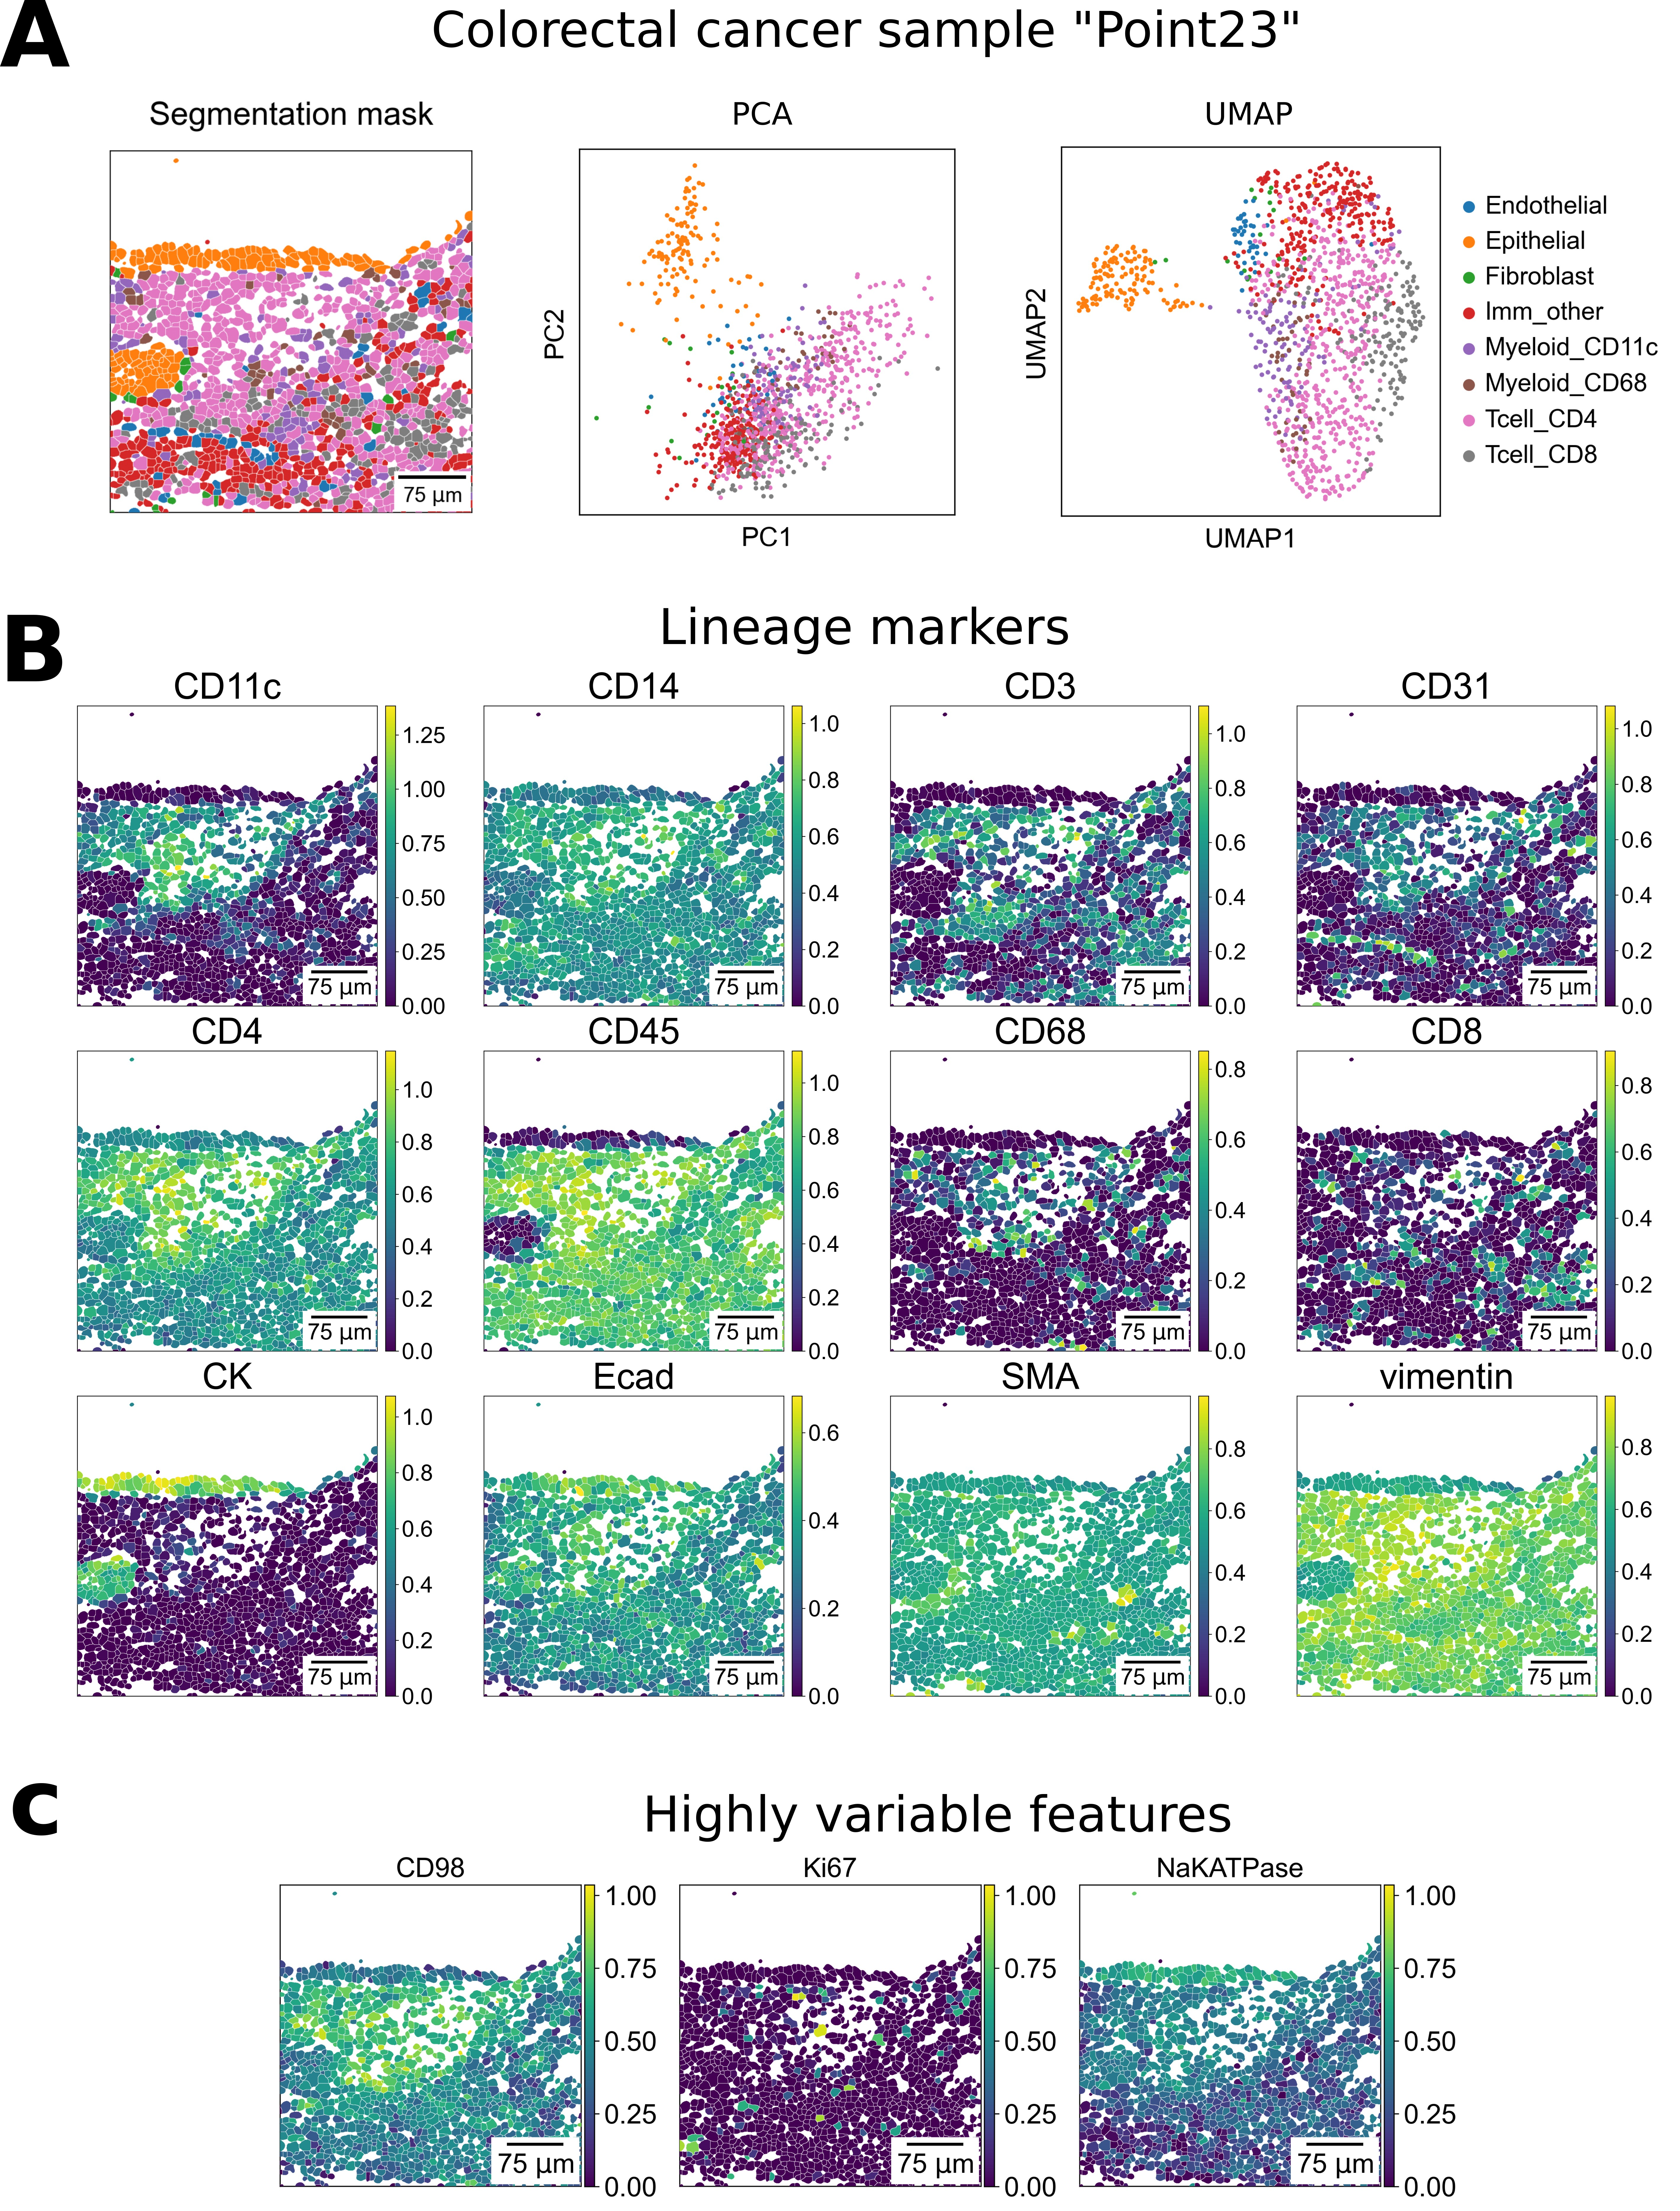
\includegraphics[width=16cm]{fig_cancer_sample_exploration}
    \caption{\textbf{Exploratory data analysis of the colorectal cancer sample "Point23".} (A) Segmentation mask, PCA and UMAP coloured by cell type. UMAP was performed on the neighbourhood graph of the first ten principal components. (B) Major immune lineage marker expression under the segmentation mask. (C) Expression of highly variable features were are not lineage markers.}
    \label{fig:explor-cancer}
\end{figure}

To contrast the characterization of the colorectal carcinoma sample, PCA and UMAP were performed on the healthy "Point49" sample (Fig. \ref{fig:explor-healthy}). Similar to the colorectal carcinoma sample, the first two components' variation only accounted for the clustering and distinction of the epithelial cell type (Fig. \ref{fig:explor-healthy}A). Upon performing UMAP on the neighbourhood graph of the first 10 principal components, the 'immune other' cell type clustered and separated from the remaining cell-types (Fig. \ref{fig:explor-healthy}B). The latter cell-types clustered but didn't separate.

Highly variable genes in the collective dataset (pooled single-cell data) were found in either the highly variable genes set of the colorectal carcinoma sample "Point 23" or the healthy sample "Point49". Accordingly, plotting the expression under the segmentation mask wasn't necessary (Fig. \ref{fig:explor-healthy}C).

\begin{figure}[p]
    \centering
    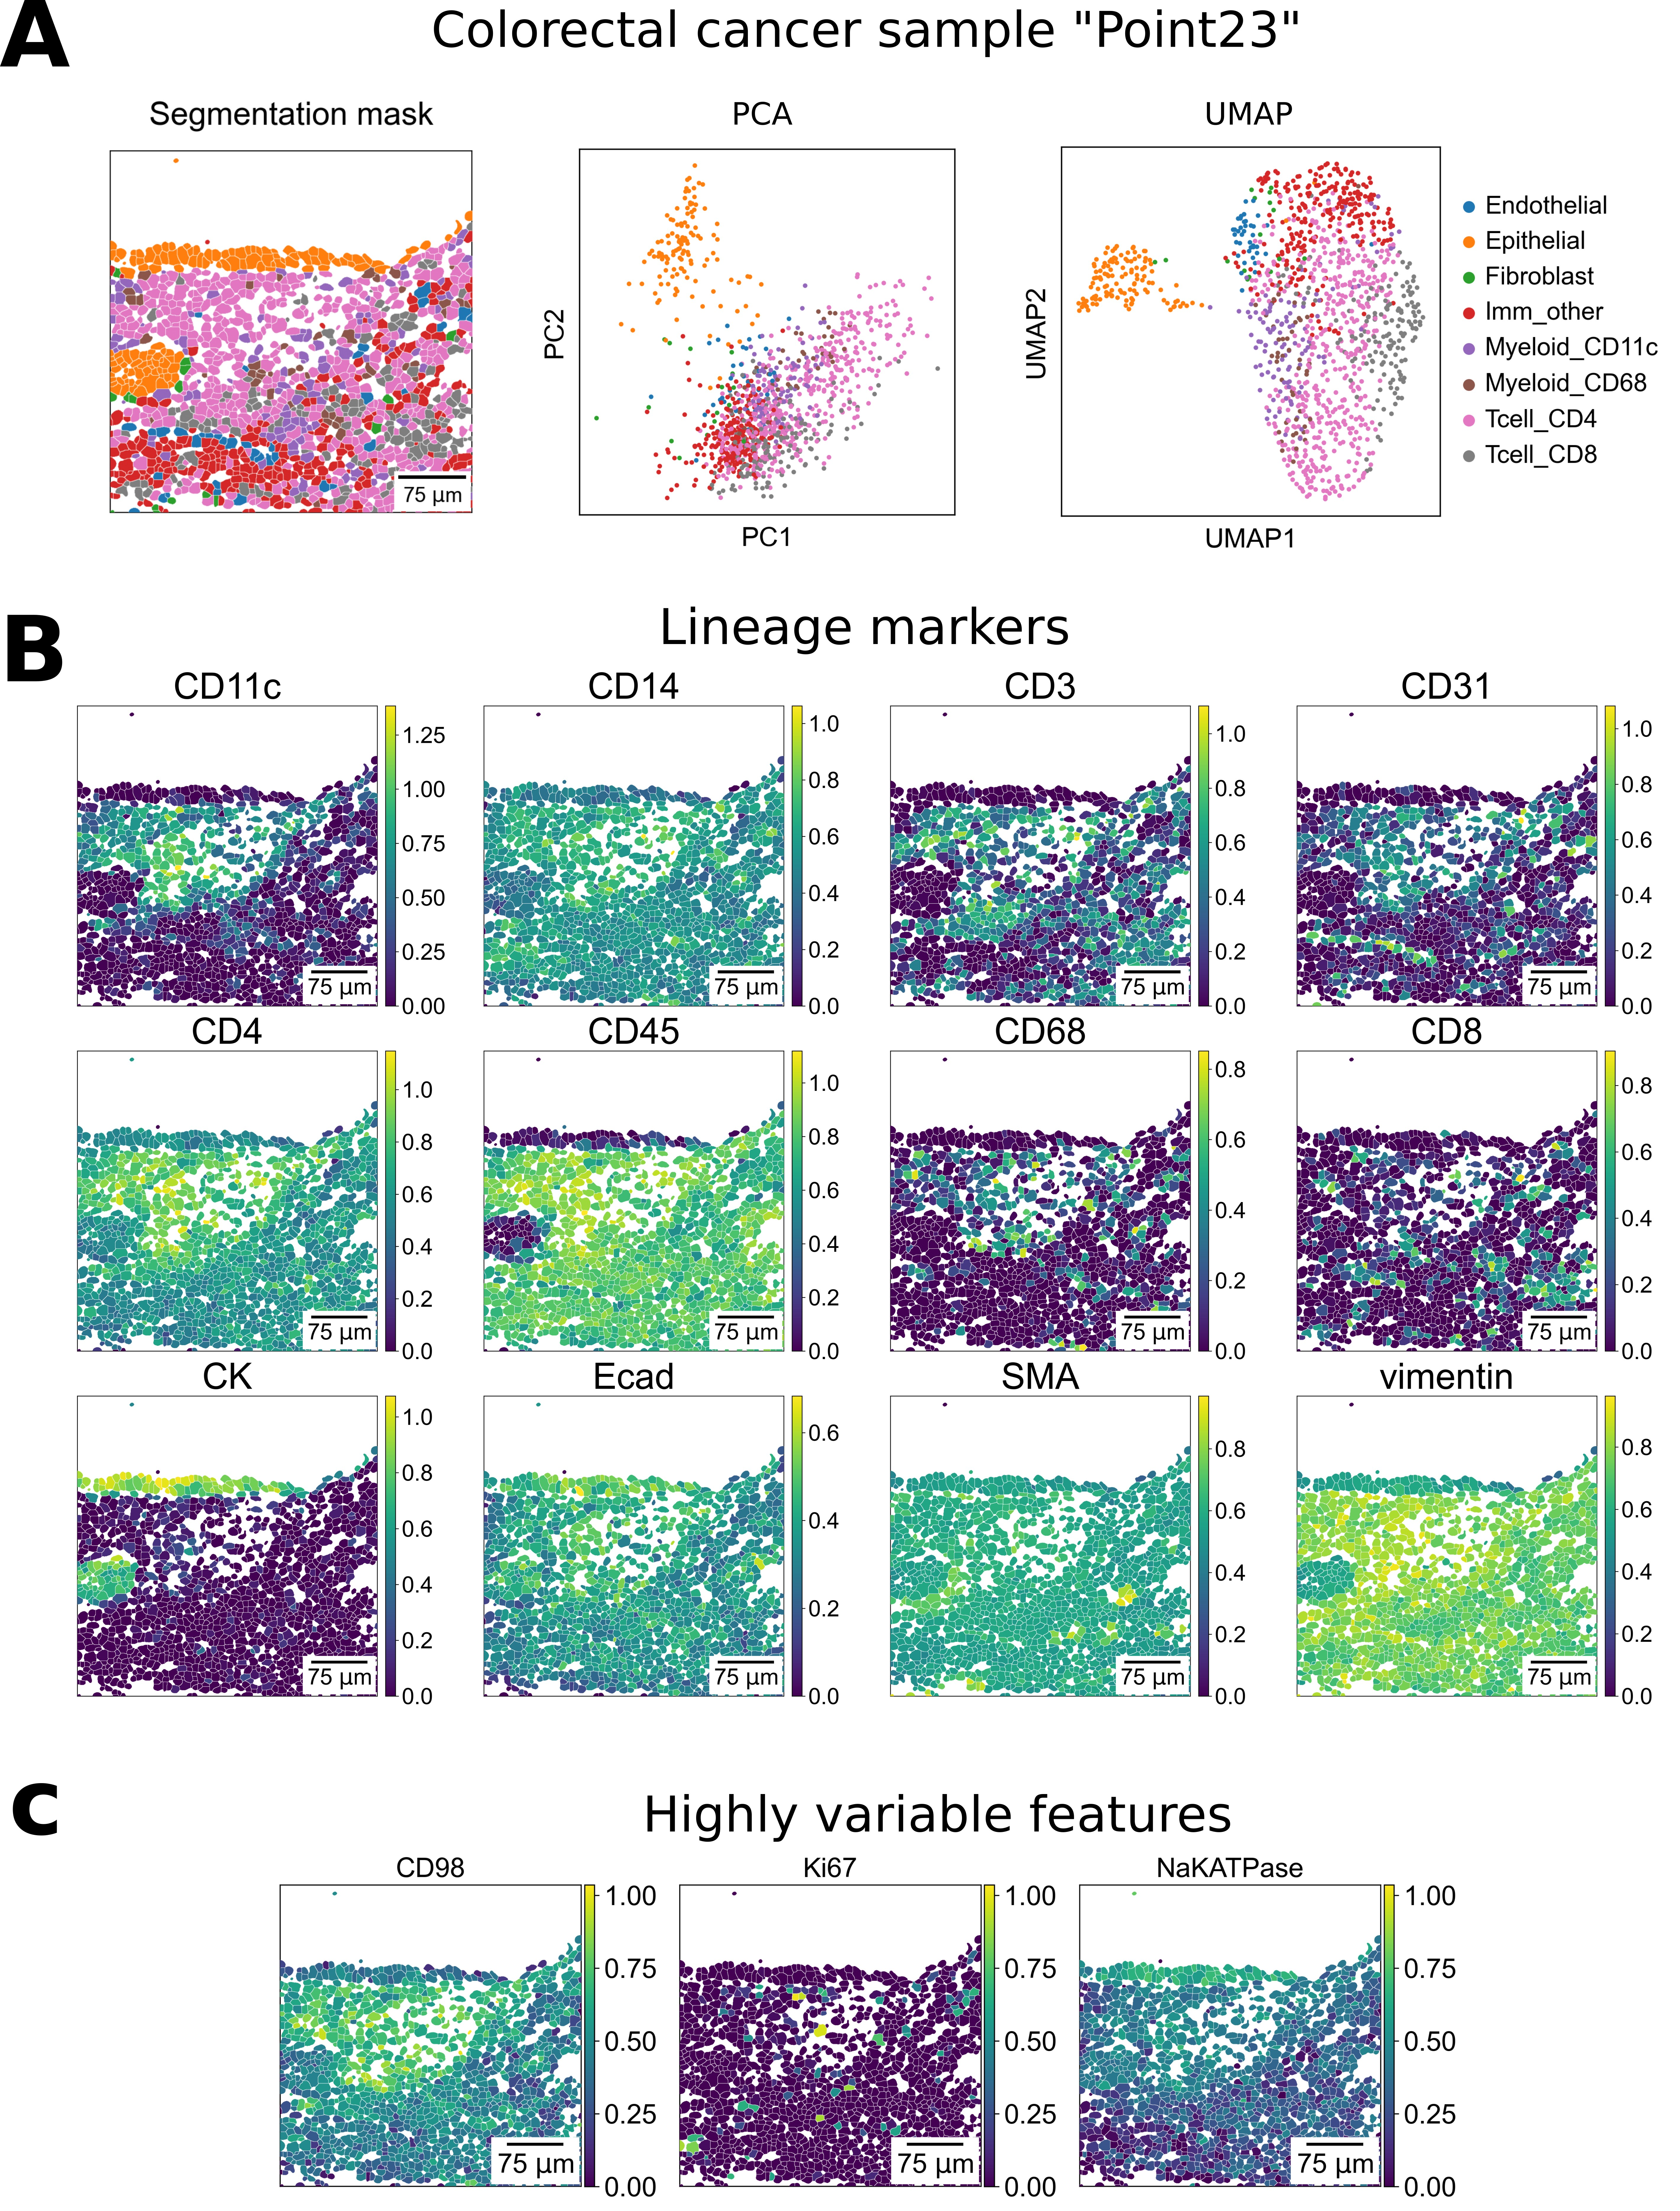
\includegraphics[width=16cm]{fig_cancer_sample_exploration}
    \caption{\textbf{Exploratory data analysis of the healthy sample "Point49".} (A) The segmentation mask coloured by cell-type and the first two dimensions of PCA and UMAP. (B) The segmentation mask of coloured by the expression levels of the major immune lineage markers. (C) Highly variable features not found within the lineage marker feature set.}
    \label{fig:explor-healthy}
\end{figure}

\pagebreak


\section{Spatial statistical analysis of cell-type distributions}

In order to investigate CCC it is important to analyze the spatial context of the the image samples on a cell-type level. This can validate or uncover tissue and niche structures as well as hint towards cell signaling on different spatial organizational levels like juxtacrine and paracrine signaling between cell types.

First the connectivity graphs of both the colorectal carcinoma sample "Point23" and the healthy sample "Point49" were calculated (Fig. \ref{fig:spatial-stats}A) by setting the neighbourhood size to a radius of 35 px (~14µm), as was calculated by \cite{Fischer-2022} to yield the best predictive performance on this dataset (explained variance, R\textsuperscript{2}) as a hole and by cell-type.

Given the anatomy of the colon, we expected a clear epithelial wall to be present in both carcinoma and healthy samples and therefore the epithelial cells to cluster. Similarly, we expected immune cells and possibly fibroblasts to aggregate close to the epithelium forming the lamina propria. Ripley's L statistic was computed to analyse the relative distribution of cells of the same annotated cell type (Fig. \ref{fig:spatial-stats}B). Indeed in both the carcinoma and healthy samples, CD4\textsuperscript{+} T cells and other CD45\textsuperscript{+} immune cells showed the highest score indicating higher relative clustering. In the carcinoma sample the CD4\textsuperscript{+} T cells had the highest score the followed by other CD45\textsuperscript{+} T cells. In the healthy sample the order was reversed. In both samples epithelial cells also showed a relatively high Ripley's L score ranked 3rd in both conditions. Furthermore, the clustering coefficient centrality scores were computed, which measure the degree of node clustering in the spatial graph for cell-type annotations. The obtained scores in the colorectal carninoma sample showed higher clustering scores in immune cells and epithelial cells compared to remaining non-immune cells (endothelial and fibroblasts) (Fig. \ref{fig:spatial-stats}C). Clustering coefficients in the healthy sample showed fibroblasts to be less clustered than the rest of the cells.

Once the clustering patterns were analyzed, relative spatial proximity between cell-types was measured via neighbourhood enrichment analysis and co-occurrence. Neighbourhood enrichment yielded in both carcinoma and healthy conditions higher values in the diagonal than other cell-type pairs (Fig. \ref{fig:spatial-stats}D). In the colorectal carcinoma sample epithelial and 'other CD45\textsuperscript{+} immune cells' showed noticeably high intra-cell-type enrichment scores indicating their respective clustering. Similarly in the healthy sample showed high enrichment of between same cell-type pairs CD4\textsuperscript{+}, CD8\textsuperscript{+} T cells and CD11c\textsuperscript{+}, CD68\textsuperscript{+} myeloid cells. Additionally CD4\textsuperscript{+} and CD8\textsuperscript{+} T cells showed to be mutually enriched. CD11c\textsuperscript{+} and CD68\textsuperscript{+} myeloid cell pairs also showed high enrichment scores. With respect to cell-type proximity to the epithelial wall, the co-occurrence score was computed for all cell-types given the presence of epithelial cells for increasing distance (Fig \ref{fig:spatial-stats} E). Applied on the colorectal carcinoma sample, it was shown that fibroblasts were more likely to be found near epithelial cells at close distance (400 px $\approx$ 156 µm) than at further distance (600 px $\approx$ 234 µm). Epithelial cell co-occurence showed high vales in this interval which declined with distance, further showing epithelial cell clustering. CD4\textsuperscript{+} and CD8\textsuperscript{+} T cells showed a constant co-occurence score while other CD45\textsuperscript{+} cells co-occurrence increase with distance to epithelial cells. Co-occurence scores on the healthy colon sample showed high values in the close range (100 px $\approx$ 39 µm) for epithelial, endothelial, CD11c\textsuperscript{+} and CD68\textsuperscript{+} myeloid cells. These scores quickly declined to a plateau at (400 px $\approx$ 156 µm). Epithelial cells had noticeably higher co-occurrence scores in at 39 µm radius indicating clustered behaviour.

\begin{figure}[p]
    \centering
    \includegraphics[width=16cm]{fig_cancer_vs_healhty_spatial-statistics_1}
\end{figure}

\begin{figure}[p]
    \centering
    \includegraphics[width=16cm]{fig_cancer_vs_healhty_spatial-statistics_2}
    \caption{\textbf{Spatial statistical analysis of annotated cell-type distribution on the spatial connectivity graph.} Colorectal carcinoma sample "Point23" localized on the left and the healthy sample "Point 49" on the right. (A) Spatial connectivity graph calculated using a radius threshold of 35 px (~14 µm). (B) Ripley's L spatial distribution statistic (C) Clustering coefficient scores computed via Squidpy (D) Neighbourhood enrichment analysis (E) Co-occurence score.}
    \label{fig:spatial-stats}
\end{figure}



\section{Spatially variable features}

In order to obtain a fuller context on a spatial level, the analysis of spatial cell-type distribution was complemented with analysis of spatially variable features on the colorectal carcinoma sample "Point23" and healthy colon sample "Point49". This was achieved via the Morans I auto-correlation statistic (Supplementary fig. \ref{tab:sup-moran}), which describes the level of dispersion and clustering of a feature across space. It was predicted that the major immune lineage markers would score a Moran's I value closer to 1 since they should enrich in their in their corresponding cell-types according to their unique profile (Fig. \ref{fig:lineage-recovery}A). In addition, highly variable genes found previously were hypothesized to show some spatial patterning. Indeed, in the colorectal cancer sample, four of the ranked features by Moran's I score were from the lineage marker set (descending order: CK, CD45, CD11c, CD4) (Fig. \ref{fig:lineage-recovery}A, \ref{fig:explor-cancer}B). Furthermore, two of the top ranked features pertained to the previously calculated highly variable features (CD98, NaKATPase) (Fig. \ref{fig:explor-cancer}C, Supplementary table \ref{tab:sup-hvargs}) and four novel features were obtained (GLUT1, HK1, LDHA, PKM2) (Fig. \ref{fig:moran}). From the top ten ranked features by Moran's I score on the healthy colon sample, 7 pertained to the major immune lineage marker set (descending order: CK, CD45, CD11c, vimentin, E-cadherin, CD14, CD3) (Fig. \ref{fig:lineage-recovery}A, \ref{fig:explor-healthy}B), 3 formed part of the preiously calculated highly variable features (CD98, Ki67, NaKATPase) (Fig. \ref{fig:explor-healthy}C, Supplementary table \ref{fig:sup1}) and no novel features with distinct expression in space were found.

\begin{figure}[h!]
    \centering
    \includegraphics[width=16cm]{fig_moransi}
    \caption{\textbf{Novel top ranked features by Moran's I score on colorectal carcinoma sample "Point23"**. Segmentation mask coloured of "Point23" coloured by the expression of features scoring top 10 in the Moran's I analysis and were not part of either the previously investigated immune lineage markers or the highly variable features calculated for the present sample.} Colorectal carcinoma sample "Point23" localized on the left and the healthy sample "Point 49" on the right. (A) Spatial connectivity graph calculated using a radius threshold of 35 px (~14 µm). (B) Ripley's L spatial distribution statistic (C) Clustering coefficient scores computed via Squidpy (D) Neighbourhood enrichment analysis (E) Co-occurence score.}
    \label{fig:moran}
\end{figure}

\pagebreak


\section{Cell-type-based sender-receiver effects calculation via NCEM interaction-terms}

Once the dataset had been characterized on the spatial and non-spatial level, the CCC methods were applied.

First, the NCEM linear model was applied to the entire dataset to obtain the interaction term coefficients, also referred to as sender-receiver effects. They are obtained asymmetrically for each sender-receiver cell-type pair and are specific to the directional interaction (dimensions: receiver cell-type x sender cell-type x features). Alongside the interaction term coefficients, FDR-corrected significance values for each interaction term were obtained for the performed Wald test.

To summarize the three-dimensional tensor, two approaches were followed. First, \cite{Fischer-2022}s approach was followed, in which the number of significant interaction terms after hypothesis testing are quantified via the L1-norm of the FDR-corrected p-value tensor. The user can set the significance threshold and an additional threshold for minimum number of obtained significant features (Fig. \ref{fig:ncem}A). Sender epithelial cells showed noticeably high interaction values on receiving CD4\textsuperscript{+} T cells. Sender CD4\textsuperscript{+} T cells showed high values when paired with CD11c, CD68 myeloid cells and other CD45\textsuperscript{+} immune cells. Other CD45\textsuperscript{+} immune cells showed high valued-interactions both as sender and receiver cells.

The second approach was aimed to be less reliant on discrete values based on a significance threshold and allow for the value of the interaction term to shape the summary statistic. This was achieved via the application of the L2-norm on the significance filtered interaction term tensor. The user can define a range- or standard-deviation-based threshold value for the used interaction terms as well as a threshold for the final L2-norm obtained values. The latter threshold can be a high-pass threshold or a percentile-based threshold. Similar to the previous significance-based approach, this approach showed a high interaction term value for the sender epithelial and receiver CD4\textsuperscript{+} cells. In contrast to the previous method, for the sender epithelial cells, a high value for the interaction with CD11c\textsuperscript{+} myeloid cells was observed. Another dissimilarity was the obtained high value for the endothelial-epithelial cell-types pair. When observing the sender effect of CD4\textsuperscript{+} T cells, their interaction coefficients on all other cell-types were not as high as in the previous approach relative to all the values in the distribution. In other words, the relative effect of CD4\textsuperscript{+} T cells on all other cells was decreased in the L2-norm approach in comparison to the significance based approach. The same relative effect reduction could also be observed on both the sender effect of 'other CD45\textsuperscript{+} immune cells' on all other cell-types and the receiver effect of 'other CD45\textsuperscript{+} immune cells' by all other immune cells. The only noticeably high values that were constant in both approaches were the 'other CD45\textsuperscript{+} immune cells' effect on CD11c\textsuperscript{+} immune cells and the receiving effect of 'other CD45\textsuperscript{+} immune cells' by CD8\textsuperscript{+} T cells.

Since the linear NCEM model is reliant on correct cell-type annotation it was hypothesized that simulating false cell-type annotation due to upstream artifacts or uncertainty in processing steps would greatly impact the output of the model. Fischer et al.'s approach to testing linear NCEM's robustness against cell segmentation error was limited to the exchange of neighbouring nodes' vectors. These, however, are often of the same cell type. Hence, it was attempted to expand on this robustness analysis by applying linear NCEM on shuffled cell-type annotations in varying fractions of random cells (fractions: 0\%, 0.1\%, 1\%, 10\%, 50\% and 100\%; shuffling repetitions for each fraction: n=15) (Fig. \ref{fig:ncem}B). As expected, the explained variance ($R^2$) already decreased in the interval between none and 1% fraction shuffling. The decrease of $R^2$  between the shuffling of 1% of the cells and 10% accounted for most of the explained variance by the model, as 50% shuffling reached the same level of $R^2$ as completely randomized cell-type annotation.

\begin{figure}[p]
    \centering
    \includegraphics[width=14cm]{fig_ncem_interactions_and_shuffling}
    \caption{\textbf{Application of linear NCEM.} (A) Sender-receiver effects obtained via two approaches. Two interaction term summary approaches (1) Quantifying the significant features per cell-type pair. The FDR-corrected p-value tensor was filtered by a significance threshold of 0.05 and the consecutively the L1-norm was calculated (Left) (2) Applying the L2-norm on the interaction terms coefficients tensor, previously filtered by a significance threshold of 0.05 (Right). (B) NCEM application on shuffled cell-type annotations by different fractions of random cells whose annotations were randomized. For each box, the center-line defines the median of the explained variance ($R^2$), the height of the box represents the inter-quartile range (IQR) and the whiskers denote the 1.5 * IQR.}
    \label{fig:ncem}
\end{figure}

\pagebreak


\section{Analysis of spatial dependencies via MISTy}

The next step was to apply MISTy to the dataset. MISTy is a predictive machine learning framework which defines "views" as spatial contexts that are to be used to predict the feature expression of the index cells. In our specific case, to not deviate too much from the NCEM concept of neighbourhoods, only one view was defined apart from the standard "intra-view". This "para-view", was constructed by adding the feature expression of cells within a certain radius 35 px (~14µm) of the index cell in a weighted manner (gaussian kernel). MISTy was run using an ensemble random forest algorithm for F().  Three types of data were collected (1) the gain of explained variance ($R^2$) achieved by comparing the $R^2$ of the model with solely the "intra-view" and the $R^2$ of the model that includes  both the "intra-view" and the "para-view" (Fig. \ref{fig:misty}A) (2) the contribution of each view to the metamodel in form of the learnable weight parameters (Fig. \ref{fig:misty}B) and (3) the improvement of the prediction of target features in the index cell via a leave-one-out procedure of predictor features in the "para-view" (Fig. \ref{fig:misty}C). MISTy was run on an individual sample level and the results where aggregated via the mean and standard deviation summary statistics.

The gain in $R^2$ of the aggregated results showed very high standard deviation, often accounting for its entire effect. SMA, PD1 and H3 were the top ranked proteins that contributed to the gain in $R^2$ by ~2.5 fold increase. Next, the results on the individual colorectal carcinoma sample "Point23" were examined yielding CD8, H3 and CD11c to be the top ranked proteins improving $R^2$ by ~3 fold. When examining the healthy colon sample "Point49", PD1, CD11c and Ki67 were the proteins that improved the $R^2$ the most by over a 4 fold increase.

The contributions of each view to the metamodel for each protein showed, as expected, that most of the contribution (consistently >50\%) comes from the "intra-view" or from the intrinsic index cell feature signaling when regarding the aggregated results. Some of the proteins that showed the highest contribution of the "para-view" were CD11c, CD8 and HIFA. In the colorectal carcinoma sample HIFA and KI67 showed a higher contribution of the "para-view" than the "intra-view". In the healthy colon sample, only CD8 showed more than half of the contribution via the "para-view". 

The feature importance results of MISTy showed sparse results in the aggregated, carcinoma sample and healthy sample results. CK was a predictor with noticeably many of the highest values across the three latter conditions. CK showed high predictive importance for target S6p, SDHA, SMA, VDAC1 in the colorectal carcinoma and healthy samples but only SDHA and SMA showed high results were high for the aggregated results. CPT1A was only high in the aggregated results. E-cadherin and citrate synthase (CS) were only high for the colorectal cancer sample and healthy sample respectively. Predictor CK was hight for ASCT2 and ATP5A in the aggregated resulst and colorectal cancer sample while only ASCT2 was high in the healthy sample. Predictor CD11c showed many high values in the colorectal carinoma and healthy samples.

\begin{figure}[hb!]
    \centering
    \includegraphics[width=8cm]{fig_misty_intra-para_r2-improvements}
\end{figure}

\begin{figure}[p]
    \centering
    \includegraphics[width=16cm]{fig_misty_intra-para_contributions-and-importances}
    \caption{\textbf{MISTy analysis of spatial dependencies by defining the "intra-" and "para-view"}. The results are shown for three categories (1) the aggregated results over all samples (Top), (2) the results on the individual colorectal carcinoma sample "Point23" (Middle) and (3) the results on the individual healthy colon sample "Point49" (Bottom). (A) Gain in variance explanation when comparing the MISTy model solely with the "intra-view" and the MISTy model including both the "intra-" and the "para-view". (B) The learnable parameters of the metamodel for each view for every feature. (C) The importances contrast heatmap. The importance of each feature to the prediction of the individual targets from the "intra-view" are subtracted from the importances calculated for the "intra-view".}
    \label{fig:misty}
\end{figure}

\pagebreak


The obtained results via MISTy were not suitable for comparison with the sender-receiver effects calculated via NCEM due to format disparity. Since the overarching goal was to to lay the groundwork for future benchmarking and evaluation of CCC methods, an approach was devised to adapt the MISTy workflow to yield comparable output. The approach consisted of transforming the input of MISTy from the feature expression matrix to the one-hot encoding matrix of the own index cells, yielding a comparable output (Fig. \ref{fig:misty_cell-types}). In essence, the prediction approach changed to predicting the index cell-type based on the neighbourhood cell-type weighted abundance. The "intra-view" was bypassed to avoid illogical prediction of cell-type within the index cell. The "para-view" was additionally modified to use a constant kernel (sum of neighbourhood cell-types across cells).

The variance explained $R^2$ was not a contrast in this case, since there was no "intra-view" to subtract. Hence it was not considered. Neither were the learnable weights results considered, since the contribution was modeled to come from the "para-view" solely.

The importances output showed no positive importance for any cell-type pair for the aggregated statistic (Fig. \ref{fig:misty_cell-types}). For the colorectal carcinoma sample, predictor endothelial cell-type showed interaction values for targets "other immune CD45\textsuperscript{+} cell", fibroblasts and CD4\textsuperscript{+} T cells.  In contrast, when examining the results on the healthy colon sample, predictor CD11c\textsuperscript{+} myeloid cells had a positive interaction value for epithelial, "other immune CD45\textsuperscript{+}", and CD4\textsuperscript{+} T cells. Also, predictor cell-type CD4\textsuperscript{+} T cells showed positive interactions with target CD11c\textsuperscript{+} myeloid, endothelial and fibroblast cells.

\begin{figure}[h!]
    \centering
    \includegraphics[width=8cm]{fig_misty_cell-types_importances}
    \caption{\textbf{MISTy workflow modified to achieve a comparable output to NCEM.} Cell-types were used as input for MISTy. Three different result categories were shown: (1) aggregated results across all samples (Top), (2) application of MISTy to colorectal carcinoma sample "Point23" (Middle) and (3) MISTy applied to healthy colon sample "Point49" (Bottom). (A) The importances heatmap of the "para-view" for each target and predictor pair.}
    \label{fig:misty_cell-types}
\end{figure}
